\documentclass[tikz,border=12pt]{standalone}
\usepackage[T1]{fontenc}
\usepackage{mathpazo}
\usepackage{amsmath,amssymb}
\usetikzlibrary{arrows.meta, positioning, calc, fit, decorations.pathreplacing}

\definecolor{stblue}{HTML}{7B97AD}
\definecolor{rwgold}{HTML}{B8995E}
\definecolor{sage}{HTML}{7A9A7E}
\definecolor{dkbrown}{HTML}{3D3530}
\definecolor{wmgray}{HTML}{7B7067}
\definecolor{cream}{HTML}{F9F6F0}
\definecolor{border}{HTML}{D4C9B8}
\definecolor{terracotta}{HTML}{C47A6A}
\definecolor{lavender}{HTML}{907EA0}

\begin{document}
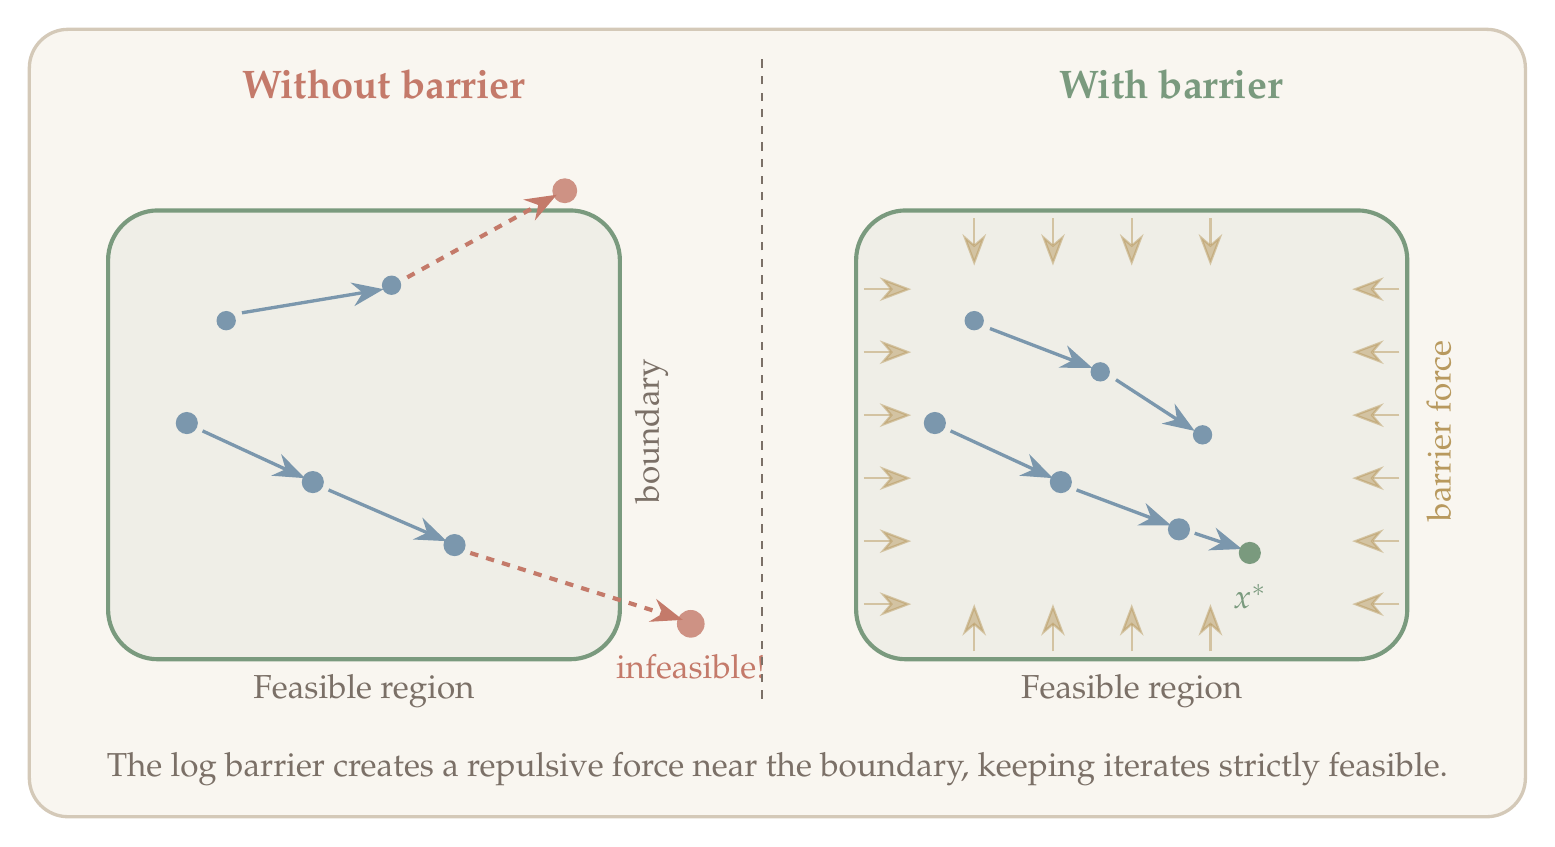
\begin{tikzpicture}[>={Stealth[length=4mm, width=3mm]}, line width=1.5pt]

% Background
\fill[cream, rounded corners=14pt] (-0.5,-1.5) rectangle (18.5,8.5);
\draw[border, line width=1.2pt, rounded corners=14pt] (-0.5,-1.5) rectangle (18.5,8.5);

%% Left Panel: Without Barrier
\node[text=terracotta, font=\Large\bfseries] at (4.0,7.8) {Without barrier};

% Feasible region
\draw[sage, line width=1.5pt, rounded corners=18pt]
  (0.5,0.5) rectangle (7.0,6.2);
\fill[sage, opacity=0.08, rounded corners=18pt]
  (0.5,0.5) rectangle (7.0,6.2);
\node[text=wmgray, font=\large] at (3.75,0.1) {Feasible region};

% Boundary label
\node[text=wmgray, font=\large, rotate=90] at (7.4,3.4) {boundary};

% Newton iterates escaping
\fill[stblue] (1.5,3.5) circle (4pt);
\draw[stblue, ->, line width=1.2pt] (1.7,3.4) -- (3.0,2.8);
\fill[stblue] (3.1,2.75) circle (4pt);
\draw[stblue, ->, line width=1.2pt] (3.3,2.65) -- (4.8,2.0);
\fill[stblue] (4.9,1.95) circle (4pt);
% Escape outside
\draw[terracotta, ->, line width=1.5pt, dashed] (5.1,1.85) -- (7.8,1.0);
\fill[terracotta, opacity=0.8] (7.9,0.95) circle (5pt);
\node[text=terracotta, font=\large] at (7.9,0.4) {infeasible!};

% Another escaping path
\fill[stblue] (2.0,4.8) circle (3.5pt);
\draw[stblue, ->, line width=1.2pt] (2.2,4.9) -- (4.0,5.2);
\fill[stblue] (4.1,5.25) circle (3.5pt);
\draw[terracotta, ->, line width=1.5pt, dashed] (4.3,5.35) -- (6.2,6.4);
\fill[terracotta, opacity=0.8] (6.3,6.45) circle (4.5pt);

% Dividing line
\draw[wmgray, dashed, line width=0.8pt] (8.8,0.0) -- (8.8,8.2);

%% Right Panel: With Barrier
\node[text=sage, font=\Large\bfseries] at (14.0,7.8) {With barrier};

% Feasible region
\draw[sage, line width=1.5pt, rounded corners=18pt]
  (10.0,0.5) rectangle (17.0,6.2);
\fill[sage, opacity=0.08, rounded corners=18pt]
  (10.0,0.5) rectangle (17.0,6.2);
\node[text=wmgray, font=\large] at (13.5,0.1) {Feasible region};

% Repulsive field lines near boundary (right side)
\foreach \y in {1.2,2.0,2.8,3.6,4.4,5.2} {
  \draw[rwgold, ->, line width=0.8pt, opacity=0.5] (16.9,\y) -- (16.3,\y);
}
% Left side
\foreach \y in {1.2,2.0,2.8,3.6,4.4,5.2} {
  \draw[rwgold, ->, line width=0.8pt, opacity=0.5] (10.1,\y) -- (10.7,\y);
}
% Top
\foreach \x in {11.5,12.5,13.5,14.5} {
  \draw[rwgold, ->, line width=0.8pt, opacity=0.5] (\x,6.1) -- (\x,5.5);
}
% Bottom
\foreach \x in {11.5,12.5,13.5,14.5} {
  \draw[rwgold, ->, line width=0.8pt, opacity=0.5] (\x,0.6) -- (\x,1.2);
}

% Barrier force label
\node[text=rwgold, font=\large, rotate=90] at (17.4,3.4) {barrier force};

% Newton iterates staying inside
\fill[stblue] (11.0,3.5) circle (4pt);
\draw[stblue, ->, line width=1.2pt] (11.2,3.4) -- (12.5,2.8);
\fill[stblue] (12.6,2.75) circle (4pt);
\draw[stblue, ->, line width=1.2pt] (12.8,2.65) -- (14.0,2.2);
\fill[stblue] (14.1,2.15) circle (4pt);
\draw[stblue, ->, line width=1.2pt] (14.3,2.1) -- (14.9,1.9);
\fill[sage] (15.0,1.85) circle (4pt);
\node[text=sage, font=\large] at (15.0,1.3) {$x^*$};

% Another path staying inside
\fill[stblue] (11.5,4.8) circle (3.5pt);
\draw[stblue, ->, line width=1.2pt] (11.7,4.7) -- (13.0,4.2);
\fill[stblue] (13.1,4.15) circle (3.5pt);
\draw[stblue, ->, line width=1.2pt] (13.3,4.05) -- (14.3,3.4);
\fill[stblue] (14.4,3.35) circle (3.5pt);

% Caption
\node[text=wmgray, font=\large] at (9.0,-0.9) {The log barrier creates a repulsive force near the boundary, keeping iterates strictly feasible.};

\end{tikzpicture}
\end{document}
